\documentclass[../main.tex]{subfiles}
\graphicspath{{\subfix{../Images}}}

\begin{document}
The e-voting system proposed in this article uses smart contracts to establish an NFT-based framework that uses these tokens as the abstractors of ballots. We use the features offered by the NFT standards indicated in Section \ref{sec:introduction_nfts} to establish mechanisms to create, edit, and transport these tokens along the system while simultaneously protecting both the identity and the choices of a voter transparently and securely. Fig. \ref{fig:general_architecture} presents a paradigm agnostic general diagram for this proposal.

\begin{figure}[htp]
    \centering
    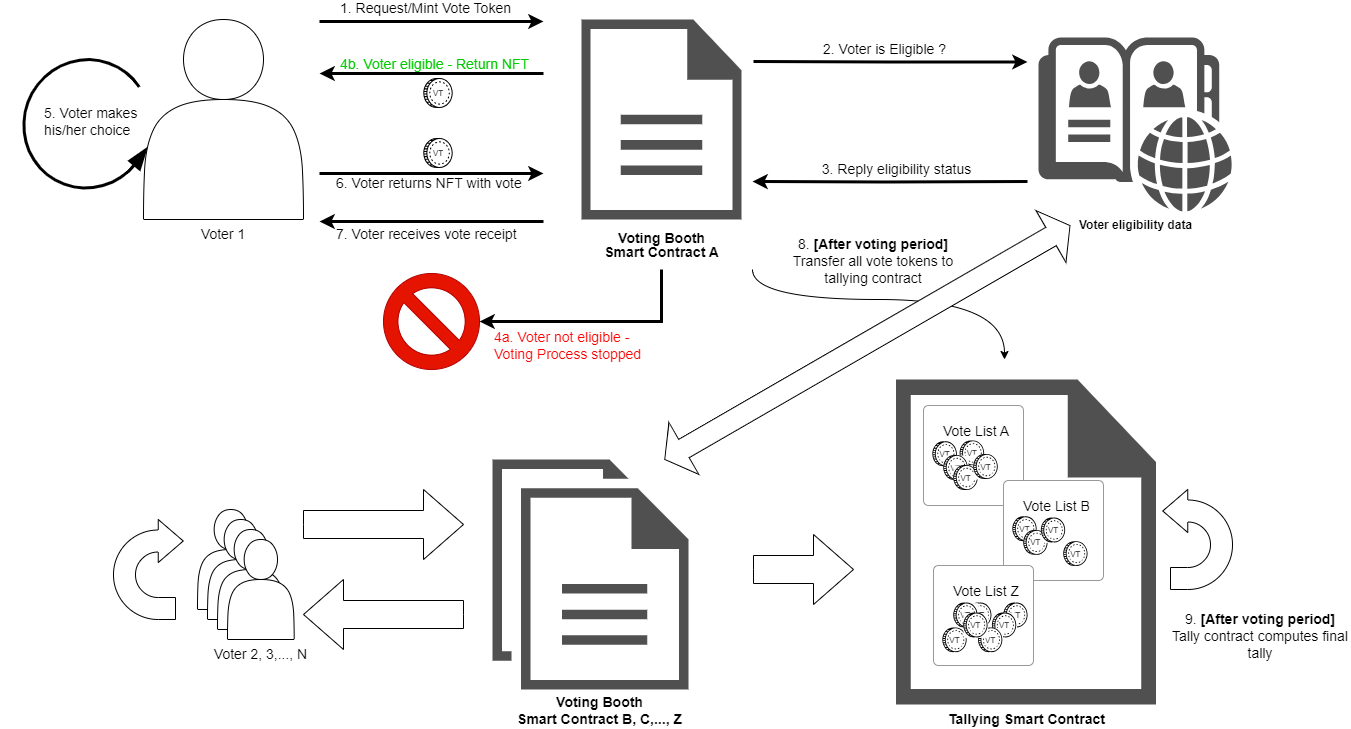
\includegraphics[width=0.7\textwidth]{../Images/01_general_solution.png}
    \caption{General architecture of an NFT-based e-voting system.}
    \label{fig:general_architecture}
\end{figure}

The proposed system is not a fully centralised one, as can be stated from Fig. \ref{fig:general_architecture}, mainly due to the intrinsically restrictive nature of elections, which typically establish \textit{a priori} rules to determine who is eligible to vote or not. The ample nature of these rules (age limit, professional background, nationality, membership in an organisation, etc.) requires the existence of a trusted third party to define and enforce them.

\subsection{Voting Process}
\begin{enumerate}
    \item{The process begins with a voter interacting with one of the voting booth smart contracts in the available set. Providing multiple points of entry into the system via the creation of multiple but functionally identical voting booth smart contracts increases availability and security by multiplying the effort that an adversary has to endure to pervert the system to his or her favour by a similar factor. Users interact with the contract by calling a public function that starts by inferring the eligibility status of the user.}

    \item{The list of eligible voters needs to be provided and managed by an external third party that regulates the election, due to the sensitive nature of most elections. For a detailed explanation of the approaches to determine voter eligibility, please refer to Section \ref{sec:voter_eligibility}, where two potential approaches that achieve the same result are detailed.}

    \item{The eligibility status determines the next course of action:
          \par
          \textbf{a.} The voter is not eligible. The process stops and informs the voter of the reason for this interruption.
          \par
          \textbf{b.} The voter is eligible. The voting booth smart contract proceeds with minting a Ballot NFT and transferring it to the voter.}

    \item{The voter makes his or her choice by editing the NFT's metadata accordingly. Editing an NFT's metadata is a relatively simple operation, but it still requires a level of technological knowledge that may be out of reach for most people. Contract functions abstract the NFT metadata edition process. This function also applies the necessary encryption layers required to preserve voter privacy. From a storage point of view, Ballot NFTs are stored under the voting booth contracts during the election period, where they can be replaced if the voter changes his or her mind, and move to the tally contract once this period ends. This process also removes the unidirectional link between the voter and his or her submitted NFT, which disables the multiple vote casting feature as well. Please refer to Section \ref{sec:multiple_vote_casting} for additional details on this feature.}

    \item{After submitting his or her choice into the Ballot NFT's metadata, the voter returns the token back to the voting boot smart contract. We make no assumptions about the storage location of this token at this point.
          \par
          The voting booth smart contract stores all Ballot NFTs whose encrypted metadata contains the choice of a voter.}

    \item{The submission of a valid vote triggers the return of a success receipt, i.e., the hash of the transaction used to return the Ballot NFT to the voting booth smart contract.}

    \item{The process described was replicated through several voting booth smart contracts used to divide the election period from the tally period, using a temporal condition to switch the functionalities available in the voting booth contracts.
          \par
          During the election period, voting booth contracts accept and validate voter requests, as well as process Ballot NFTs for successful voter requests. The end of the election period triggers the start of the tally period. During it, voting booth contracts refuse voter requests by default, either to mint a Ballot NFT or to submit a previously minted token, while they transfer all stored tokens thus far to a tally contract.
          \par
          With all Ballot NFTs under the control of the tallying smart contract, the counting can begin once the data is ready, i.e., all encryption layers and randomising elements (salt) are removed from the vote data.
          \par
          Once finished, another public contract function retrieves the final tally. The contract stores the tally results for future reference and auditing purposes.}
\end{enumerate}

The general approach described morphs into two different systems depending on the type of data storage paradigm employed by the blockchain used to implement this system. Sections \ref{sec:contract-based-approach} and \ref{sec:account-based-approach} detail the two options in greater detail.

\section{Contract-based Approach}
\label{sec:contract-based-approach}
\subfile{./06_ContractBasedApproach.tex}

\section{Account-based Approach}
\label{sec:account-based-approach}
\subfile{./07_AccountBasedApproach.tex}
\end{document}